\chapter{Registration}

This chapter introduces the funtionalities offered by Insight for performing
image registration. Image registration is the process in which we determine
the spatial transform that maps points from one image to homologous points
on the object in the second image. In the toolkit, registration is performed 
within a framework of pluggable components that can easily be interchanged. 
This flexibility means that a combinatorial variety of registration methods can
be created, allowing the user to pick and choose the right tools for 
the application.

\section{Registration Framework}
The components of the registration framework and their interconnections 
are shown in Figure \ref{fig:RegistrationComponents}. The basic
input data to the registration process are two images: one
is defined as the \emph{Fixed} image $f(\bf{X})$ and the other defined as the
\emph{Moving} image $m(\bf{X})$. Registration is treated as an optimization problem
with the goal of finding the spatial mapping that will bring the moving image into 
alignment with the fixed or target image.

\begin{figure}
\center
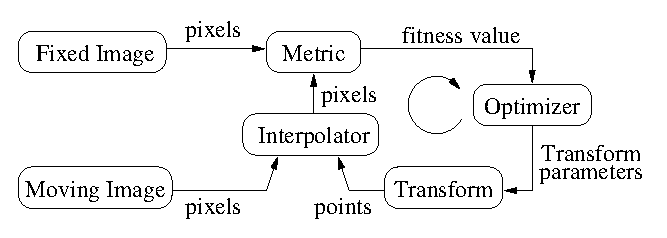
\includegraphics[width=12cm]{RegistrationComponentsDiagram.eps}
\caption{The basic components of the registration framework are two input images,
a transform, a metric, an interpolator and an optimizer.}
\label{fig:RegistrationComponents}
\end{figure}

The \emph{Transform} component $T(\bf{X})$ represents the spatial mapping of points 
from the fixed image space to points in the moving image space. Note that this 
definition is inverse to the usual view of image transformation. Using the
\emph{inverse} transform is typical in registration as it avoids the potential
problems of "holes" with forward transform. The \emph{Interpolator} is used to
evaluate moving image intensity at non-grid positions. The \emph{Metric} component
$S(f,m \circ T)$ provides a measure of how well the fixed image is matched by 
the transformed moving image. This measure forms the quantitative criterion to be optimized 
by the \emph{Optimizer} over the search space defined by the parameters of the 
\emph{Transform}.

The various components available in the toolkit will be described in later sections.
First we begin with a simple registration example.

\section{Hello World Registration}
\label{sec:IntroductionImageRegistration}
\input{ImageRegistration1.tex}


\section{Transforms}
\label{sec:Transforms}
\input{Transform.tex}

\section{Interpolators}
\label{sec:Interpolators}
%
%  This file is included by Registration.tex
%

\begin{figure}
\centering
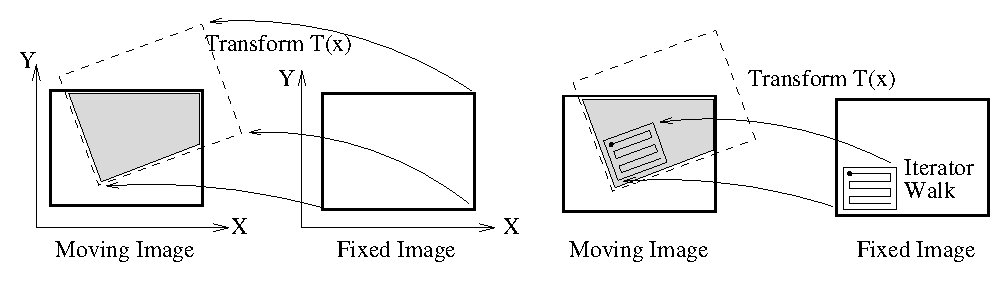
\includegraphics[width=\textwidth]{ImageOverlap.eps}
\itkcaption[Mapping moving image to fixed image in Registration]{ The moving
image is mapped into the fixed image space under some spatial
transformation. An iterator walks through the fixed image and its coordinates
are mapped onto the moving image.}
\label{fig:ImageOverlapIterator}
\end{figure}


\begin{floatingfigure}[rlp]{0.5\textwidth}
 \centering
 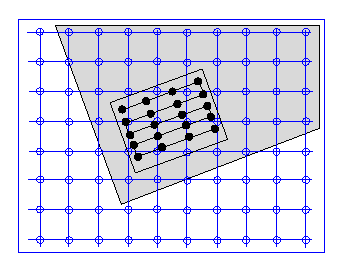
\includegraphics[width=7.5cm]{ImageOverlapInterpolator.eps}
 \caption[Need for interpolation in Registration]{Grid positions of the fixed
image map to non-grid positions of the moving
image.  \label{fig:ImageOverlapInterpolator}}
\end{floatingfigure}

In the registration process, the metric typically compares intensity values
in the fixed image against the corresponding values in the transformed moving
image. When a point is mapped from one space to another by a transform, it
will in general be mapped to a non-grid position. Therefore, interpolation is
required to evaluate the image intensity at the mapped position.

Figure \ref{fig:ImageOverlapIterator} (left) illustrates the mapping of the
fixed image space onto the moving image space. The transform maps points from
the fixed image coordinate system onto the moving image coordinate system. The
figure highlights the region of overlap between the two images after the
mapping. The right side illustrates how an iterator is used to walk through a
region of the fixed image. Each one of the iterator positions is mapped by the
transform onto the moving image space in order to find the homologous pixel.

Figure \ref{fig:ImageOverlapInterpolator} presents a detailed view of the
mapping from the fixed image to the moving image. In general, the grid
positions of the fixed image will not be mapped onto grid positions of the
moving image.  Interpolation is needed for estimating the intensity of the
moving image at these non-grid positions. The service is provided in ITK by
interpolator classes that can be plugged into the registration method.

\index{Nearest\-Neighbor\-Interpolate\-Image\-Function}
\index{Linear\-Interpolate\-Image\-Function}
\index{BSpline\-Interpolate\-Image\-Function}
\index{Windowed\-Sinc\-Interpolate\-Image\-Function}

The following interpolators are available:

\begin{itemize}
\item \doxygen{NearestNeighborInterpolateImageFunction}
\item \doxygen{LinearInterpolateImageFunction}
\item \doxygen{BSplineInterpolateImageFunction}
\item \doxygen{WindowedSincInterpolateImageFunction}
\end{itemize}

In the context of registration, the interpolation method affects the smoothness
of the optimization search space and the overall computation time. On the other
hand, interpolations are executed thousands of times in a single optimization
cycle. Hence, the user has to balance the simplicity of computation with the
smoothness of the optimization when selecting the interpolation scheme.

\index{itk::InterpolateImageFunction}
\index{itk::InterpolateImageFunction!SetInputImage()}
\index{itk::InterpolateImageFunction!Evaluate()}
\index{itk::InterpolateImageFunction!EvaluateAtContinuousIndex()}
\index{itk::InterpolateImageFunction!IsInsideBuffer()}

The basic input to an \doxygen{InterpolateImageFunction} is the image to
be interpolated. Once an image has been defined using \code{SetInputImage()},
a user can interpolate either at a point using \code{Evaluate()} or
an index using \code{EvaluateAtContinuousIndex()}.

Interpolators provide the method \code{IsInsideBuffer()} that tests whether a
particular image index or a physical point falls inside the spatial domain for
which image pixels exist.

\subsection{Nearest Neighbor Interpolation}
\label{sec:NearestNeighborInterpolation}
\index{itk::Nearest\-Neighbor\-Interpolate\-Image\-Function}
The \doxygen{NearestNeighborInterpolateImageFunction} simply uses the
intensity of the nearest grid position. That is, it assumes that the image
intensity is piecewise constant with jumps mid-way between grid positions.
This interpolation scheme is cheap as it does not require any floating point
computations.


\subsection{Linear Interpolation}
\label{sec:LinearInterpolation}
\index{itk::Linear\-Interpolate\-Image\-Function}

The \doxygen{LinearInterpolateImageFunction} assumes that intensity varies
linearly between grid positions. Unlike nearest neighbor interpolation, the
interpolated intensity is spatially continuous. However, the intensity
gradient will be discontinuous at grid positions.


\subsection{B-Spline Interpolation}
\label{sec:BSplineInterpolation}
\index{itk::BSpline\-Interpolate\-Image\-Function}

\begin{figure}
\center
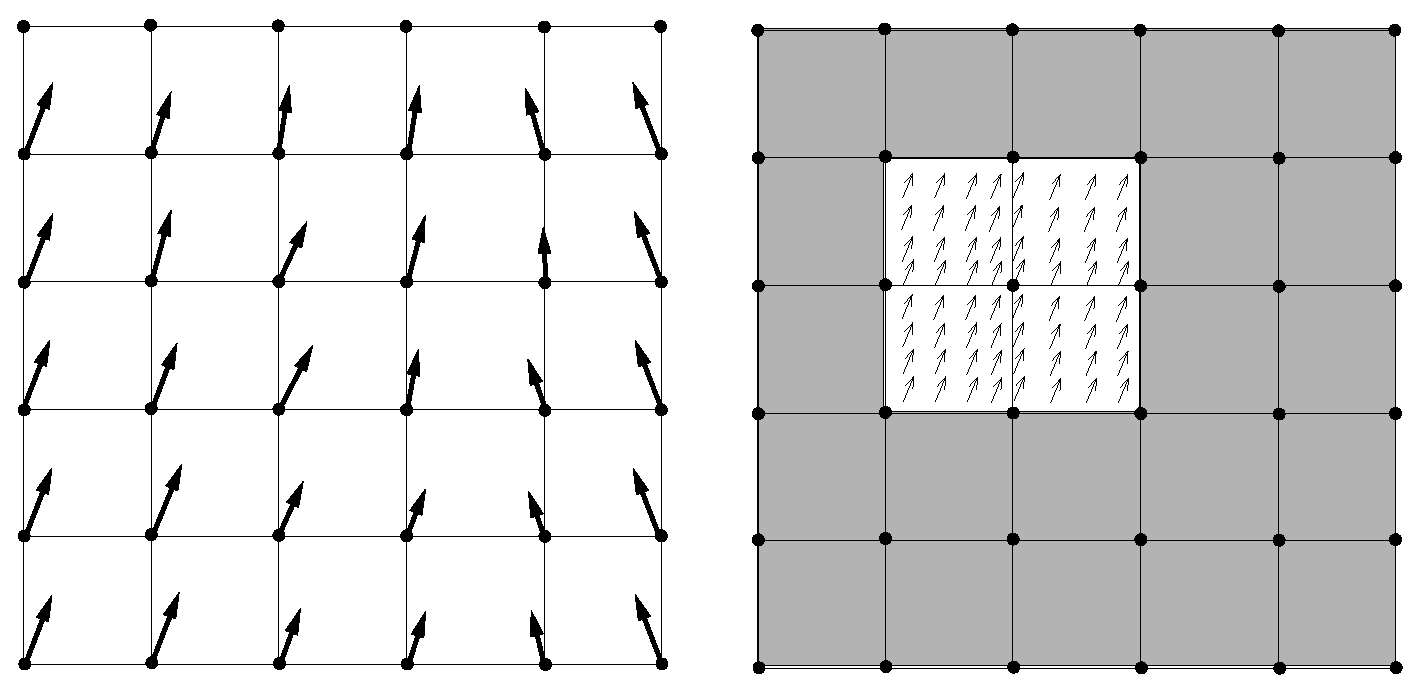
\includegraphics[width=0.9\textwidth]{BSplineInterpolation.eps}
\itkcaption[BSpline Interpolation Concepts]{The left side illustrates the
BSpline grid and the deformations that are known on those nodes. The right side
illustrates the region where interpolation is possible when the BSpline is of
cubic order. The small arrows represent deformation values that were
interpolated from the grid deformations shown on the left side of the diagram.}
\label{fig:BSplineInterpolation}
\end{figure}


The \doxygen{BSplineInterpolateImageFunction} represents the image intensity
using B-spline basis functions. When an input image is first connected to the
interpolator, B-spline coefficients are computed using recursive filtering
(assuming mirror boundary conditions). Intensity at a non-grid position is
computed by multiplying the B-spline coefficients with shifted B-spline kernels
within a small support region of the requested position.
Figure~\ref{fig:BSplineInterpolation} illustrates on the left how the
deformation values on the BSpline grid nodes are used for computing
interpolated deformations in the rest of space. Note for example that when a
cubic BSpline is used, the grid must have one extra node in one side of the
image and two extra nodes on the other side, this along every dimension.

Currently, this interpolator supports splines of order $0$ to $5$. Using a
spline of order $0$ is almost identical to nearest neighbor interpolation; a
spline of order $1$ is exactly identical to linear interpolation. For splines
of order greater than $1$, both the interpolated value and its derivative are
spatially continuous.

It is important to note that when using this scheme, the interpolated
value may lie outside the range of input image intensities. This is
especially important when handling unsigned data, as it is possible
that the interpolated value is negative.


\subsection{Windowed Sinc Interpolation}
\label{sec:WindowedSincInterpolation}
\index{itk::Windowed\-Sinc\-Interpolate\-Image\-Function}

The \doxygen{WindowedSincInterpolateImageFunction} is the best possible
interpolator for data that have been digitized in a discrete grid. This
interpolator has been developed based on Fourier Analysis considerations. It
is well known in signal processing that the process of sampling a spatial
function using a periodic discrete grid results in a replication of the
spectrum of that signal in the frequency domain.

The process of recovering the continuous signal from the discrete sampling is
equivalent to the removal of the replicated spectra in the frequency domain.
This can be done by multiplying the spectra with a box function that will set
to zero all the frequencies above the highest frequency in the original signal.
Multiplying the spectrum with a box function is equivalent to convolving the
spatial discrete signal with a sinc function

\begin{equation}
sinc(x) = \sin{(x)} / x
\end{equation}

The sinc function has infinite support, which of course in practice can not
really be implemented. Therefore, the sinc is usually truncated by multiplying
it with a Window function. The Windowed Sinc interpolator is the result of such an
operation.

This interpolator presents a series of trade-offs in its utilization. Probably
the most significant is that the larger the window, the more precise will be
the resulting interpolation. However, large windows will also result in long
computation times. Since the user can select the window size in this
interpolator, it is up to the user to determine how much interpolation quality
is required in her/his application and how much computation time can be
justified. For details on the signal processing theory behind this
interpolator, please refer to Meijering \emph{et.
al}~\cite{SignalReconstruction}.

The region of the image used for computing the interpolator is determined by
the window \emph{radius}. For example, in a $2D$ image where we want to
interpolate the value at position $(x,y)$ the following computation will be
performed.

\begin{equation}
I(x,y) =
\sum_{i = \lfloor x \rfloor + 1 - m}^{\lfloor x \rfloor + m}
\sum_{j = \lfloor y \rfloor + 1 - m}^{\lfloor y \rfloor + m}
I_{i,j} K(x-i) K(y-j)
\end{equation}

where $m$ is the \emph{radius} of the window. Typically, values such as 3 or 4
are reasonable for the window radius. The function kernel $K(t)$ is composed by
the $sinc$ function and one of the windows listed above.

\begin{equation}
K(t) = w(t) \textrm{sinc}(t) = w(t) \frac{\sin(\pi t)}{\pi t}
\end{equation}

Some of the windows that can be used with this interpolator are

Cosinus window
\begin{equation}
w(x) = cos ( \frac{\pi x}{2 m} )
\end{equation}


Hamming window
\begin{equation}
w(x) = 0.54 + 0.46 cos ( \frac{\pi x}{m} )
\end{equation}


Welch window
\begin{equation}
w(x) = 1 - ( \frac{x^2}{m^2} )
\end{equation}


Lancos window
\begin{equation}
w(x) = \textrm{sinc} ( \frac{x}{m} )
\end{equation}


Blackman window
\begin{equation}
w(x) = 0.42 + 0.5 cos(\frac{\pi x}{m}) + 0.08 cos(\frac{2 \pi x}{m})
\end{equation}


The window functions listed above are available inside the itk::Function
namespace. The conclusions of the referenced paper suggest to use the Welch,
Cosine, Kaiser, and Lancos windows for m = 4,5. These are based on error in
rotating medical images with respect to the linear interpolation method. In
some cases the results achieve a 20-fold improvement in accuracy.

This filter can be used in the same way you would use any
ImageInterpolationFunction. For instance, you can plug it into the
ResampleImageFilter class.  In order to instantiate the filter you must choose
several template parameters.

\small
\begin{minted}[baselinestretch=1,fontsize=\footnotesize,linenos=false,bgcolor=ltgray]{c++}
using InterpolatorType = WindowedSincInterpolateImageFunction<
           TInputImage, VRadius, TWindowFunction,
           TBoundaryCondition, TCoordRep >;

\end{minted}
\normalsize

\code{TInputImage} is the image type, as for any other interpolator.

\code{VRadius} is the radius of the kernel, i.e., the $m$ from the
formula above.

\code{TWindowFunction} is the window function object, which you can choose from
about five different functions defined in this header. The default is the
Hamming window, which is commonly used but not optimal according to the cited
paper.

\code{TBoundaryCondition} is the boundary condition class used to determine the
values of pixels that fall off the image boundary. This class has the same
meaning here as in the \doxygen{NeighborhoodIterator} classes.

\code{TCoordRep} is again standard for interpolating functions, and should be
float or double.


The WindowedSincInterpolateImageFunction is probably not the interpolator that
you want to use for performing registration. Its computation burden makes it
too expensive for this purpose. The best use of this interpolator is for the
final resampling of the image, once the transform has been found using
another less expensive interpolator in the registration process.


\section{Metrics}
\label{sec:Metrics}
%
%  This file is included by Registration.tex
%
%
%

\index{itk::Image\-To\-Image\-Metric}

In ITK, \doxygen{ImageToImageMetric} objects quantitatively measure how well
the transformed moving image fits the fixed image by comparing the gray-scale
intensity of the images. These metrics are very flexible and can work with any
transform or interpolation method and do not require reduction of the
gray-scale images to sparse extracted information such as edges.

The metric component is perhaps the most critical element of the registration
framework. The selection of which metric to use is highly dependent on the
registration problem to be solved. For example, some metrics have a large
capture range while others require initialization close to the optimal
position.  In addition, some metrics are only suitable for comparing images 
obtained from the same imaging modality, while others can handle 
inter-modality comparisons.
Unfortunately, there are no clear-cut rules as to how to choose a metric.

\index{itk::Image\-To\-Image\-Metric!GetValue()}
\index{itk::Image\-To\-Image\-Metric!GetDerivatives()}
\index{itk::Image\-To\-Image\-Metric!GetValueAndDerivatives()}

The basic inputs to a metric are: the fixed and moving images, a transform and
an interpolator. The method \code{GetValue()} can be used to evaluate the
quantitative criterion at the transform parameters specified in the argument.
Typically, the metric samples points within a defined region of the fixed
image.  For each point, the corresponding moving image position is computed
using the transform with the specified parameters, then the interpolator is
used to compute the moving image intensity at the mapped position. Details on
this mapping are illustrated in Figures \ref{fig:ImageOverlapIterator} and
\ref{fig:ImageOverlapInterpolator}. 

The metrics also support region based evaluation. The \code{SetFixedImageMask()} and 
\code{SetMovingImageMask()} methods may be used to restrict evaluation of the metric 
within a specified region. The masks may be of any type derived from \doxygen{SpatialObject}.

Besides the measure value, gradient-based optimization schemes also require
derivatives of the measure with respect to each transform parameter. The
methods \code{GetDerivatives()} and \code{GetValueAndDerivatives()} can be
used to obtain the gradient information.


The following is the list of metrics currently available in ITK:
\begin{itemize}
\item mean squares\\ \doxygen{MeanSquaresImageToImageMetric}
\item normalized correlation \\ \doxygen{NormalizedCorrelationImageToImageMetric}
\item mean reciprocal squared difference \\ \doxygen{MeanReciprocalSquareDifferenceImageToImageMetric} 
\item mutual information by Viola and Wells \\ \doxygen{MutualInformationImageToImageMetric}
\item mutual information by Mattes \\ \doxygen{MattesMutualInformationImageToImageMetric}
\item Kullback Liebler distance metric by Kullback and Liebler \\ \doxygen{KullbackLeiblerCompareHistogramImageToImageMetric}
\item Normalized mutual information \\ \doxygen{NormalizedMutualInformationHistogramImageToImageMetric}
\item Cardinality Match metric \\ \doxygen{MatchCardinalityImageToImageMetric}
\item Kappa Statistics metric\\ \doxygen{KappaStatisticImageToImageMetric}
\item Gradient Difference metric \\ \doxygen{GradientDifferenceImageToImageMetric}
\end{itemize}

In the following sections, we describe each metric type in detail. 
For ease of notation, we will refer to the fixed image $f(\bf{X})$ 
and transformed moving image $(m \circ T(\bf{X}))$ as images $A$ and $B$.

\subsection{Mean Squares Metric}
\label{sec:MeanSquaresMetric}
\index{itk::Mean\-Squares\-Image\-To\-Image\-Metric}

The \doxygen{MeanSquaresImageToImageMetric} computes the mean squared
pixel-wise difference in intensity between image $A$ and $B$ over a user
defined region:

\begin{equation}
MS(A,B) = \frac{1}{N} \sum_{i=1}^N \left( A_i - B_i \right)^2
\end{equation}
\begin{center}
$A_i$ is the i-th pixel of Image A\\ 
$B_i$ is the i-th pixel of Image B\\
$N$ is the number of pixels considered
\end{center}

The optimal value of the metric is zero. Poor matches between images $A$ and
$B$ result in large values of the metric. This metric is simple to compute and
has a relatively large capture radius.

This metric relies on the assumption that intensity representing the same
homologous point must be the same in both images. Hence, its use is restricted
to images of the same modality. Additionally, any linear changes in the
intensity result in a poor match value.

\subsubsection{Exploring a Metric}
\label{sec:ExploringAMetric}

Getting familiar with the characteristics of the Metric as a cost function is
fundamental in order to find the best way of seting up an optimization process
that will use this metric for solving a registration problem. 

\ifitkFullVersion
\input{MeanSquaresImageMetric1.tex}
\fi


\subsection{Normalized Correlation Metric}
\label{sec:NormalizedCorrelationMetric}
\index{itk::Normalized\-Correlation\-Image\-To\-Image\-Metric}

The \doxygen{NormalizedCorrelationImageToImageMetric} computes pixel-wise
cross-correlation and normalizes it by the square root of the autocorrelation
of the images:

\begin{equation}
NC(A,B) = -1 \times \frac{ \sum_{i=1}^N \left( A_i \cdot B_i \right) }
        { \sqrt { \sum_{i=1}^N A_i^2  \cdot \sum_{i=1}^N B_i^2 } }
\end{equation}
\begin{center}
$A_i$ is the i-th pixel of Image A\\ 
$B_i$ is the i-th pixel of Image B\\
$N$ is the number of pixels considered
\end{center}

Note the $-1$ factor in the metric computation. This factor is used to make the
metric be optimal when its minimum is reached.  The optimal value of the metric
is then minus one. Misalignment between the images results in small measure
values.  The use of this metric is limited to images obtained using the same
imaging modality.  The metric is insensitive to multiplicative factors between
the two images.  This metric produces a cost function with sharp peaks and well
defined minima.  On the other hand, it has a relatively small capture radius.

\subsection{Mean Reciprocal Square Differences}
\label{sec:MeanReciprocalSquareDifferenceMetric}
\index{itk::Mean\-Reciprocal\-Square\-Difference\-Image\-To\-Image\-Metric}

The \doxygen{MeanReciprocalSquareDifferenceImageToImageMetric} computes
pixel-wise differences and adds them after passing them through a bell-shaped
function $\frac{1}{1+x^2}$:

\begin{equation}
PI(A,B) =  \sum_{i=1}^N \frac{ 1 }{ 1 + \frac{ \left( A_i - B_i \right) ^ 2}{ \lambda^2 }  }
\end{equation}
\begin{center}
$A_i$ is the i-th pixel of Image A \\
$B_i$ is the i-th pixel of Image B \\
$N$ is the number of pixels considered \\
$\lambda$ controls the capture radius
\end{center}

The optimal value is $N$ and poor matches results in small measure values.
The characteristics of this metric have been studied by Penney and Holden
\cite{Holden1999}\cite{Penney1998}

This image metric has the advantage of producing poor values when few pixels
are considered.  This makes it consistent when its computation is subject to
the size of the overlap region between the images. The capture radius of the
metric can be regulated with the parameter $\lambda$.  The profile of this
metric is very peaky. The sharp peaks of the metric help to measure spatial
misalignment with high precision. Note that the notion of capture radius is
used here in terms of the intensity domain, not the spatial domain. In that
regard, $\lambda$ should be given in intensity units and be associated with
the differences in intensity that will make drop the metric by $50\%$.

The metric is limited to images of the same image modality.  The
fact that its derivative is large at the central peak is a problem for some
optimizers that rely on the derivative to decrease as the extrema are
reached.  This metric is also sensitive to linear changes in intensity.


\subsection{Mutual Information Metric}
\label{sec:MutualInformationMetric}

The \doxygen{MutualInformationImageToImageMetric} computes the mutual
information between image $A$ and image $B$.  Mutual information (MI)
measures how much information one random variable (image intensity in one
image) tells about another random variable (image intensity in the other
image). The major advantage of using MI is that the actual form of the
dependency does not have to be specified.  Therefore, complex mapping between
two images can be modeled.  This flexibility makes MI well suited as a
criterion of multi-modality registration~\cite{Pluim2003}.

Mutual information is defined in terms of entropy. Let
\begin{equation}
H(A) = - \int p_A(a) \log p_A(a)\, da
\end{equation}
be the entropy of random variable $A$, $H(B)$ the entropy of 
random variable $B$ and 
\begin{equation}
H(A,B) = \int p_{AB}(a,b) \log p_{AB}(a,b)\,da\,db
\end{equation}
be the joint entropy of $A$ and $B$. If $A$ and $B$ are independent, then
\begin{equation}
p_{AB}(a,b) = p_A(a) p_B(b)
\end{equation}
and
\begin{equation}
H(A,B) = H(A) + H(B).
\end{equation}
However, if there is any dependency, then
\begin{equation}
H(A,B)<H(A)+H(B).
\end{equation}
The difference is called Mutual Information : \( I(A,B) \)
\begin{equation}
I(A,B)=H(A)+H(B)-H(A,B)
\end{equation}

\subsubsection{Parzen Windowing}

\itkpiccaption[Parzen Windowing in Mutual Information]{
In Parzen windowing, a continuous density function is constructed by
superimposing kernel functions (Gaussian function in this case) centered on the
intensity samples obtained from the image.\label{fig:ParzenWindowing}}
\parpic(0.5\textwidth,5.5cm)[r]{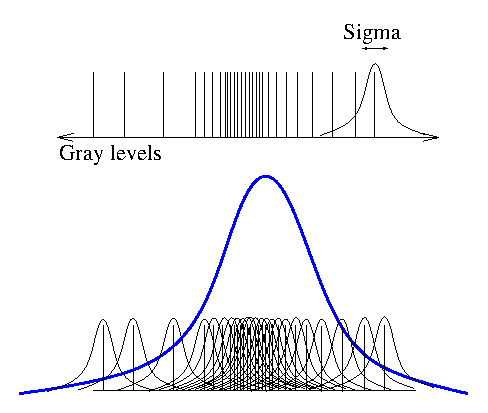
\includegraphics[width=0.48\textwidth]{ParzenWindowing13.eps}}

In a typical registration problem, direct access to the marginal 
and joint probability densities is not available and hence the
densities must be estimated from the image data. Parzen windows 
(also known as kernel density estimators) can be used for this purpose.
In this scheme, the densities are constructed by taking intensity 
samples $S$ from the image and super-positioning kernel functions 
$K(\cdot)$ centered on the elements of $S$ as illustrated in
Figure \ref{fig:ParzenWindowing}:

A variety of functions can be used as the smoothing kernel with the
requirement that they are smooth, symmetric, have zero mean and
integrate to one. For example, boxcar, Gaussian and B-spline functions are
suitable candidates.  A smoothing parameter is used to scale the kernel
function.  The larger the smoothing parameter, the wider the kernel function
used and hence the smoother the density estimate. If the parameter is too
large, features such as modes in the density will get smoothed out.  On the
other hand, if the smoothing parameter is too small, the resulting density
may be too noisy. The estimation is given by the following equation.

\begin{equation}
p(a) \approx P^{*}(a) = \frac{1}{N} \sum_{s_j \in S} K\left(a - s_j\right)
\end{equation}

Choosing the optimal smoothing parameter is a difficult research problem and
beyond the scope of this software guide.  Typically, the optimal value of the
smoothing parameter will depend on the data and the number of samples used.

\subsubsection{Viola and Wells Implementation}

The Insight Toolkit has two mutual information metric implementations. The
first is \doxygen{MutualInformationImageToImageMetric} and follows the method
specified by Viola and Wells in \cite{Viola1997}.

\index{itk::Mutual\-Information\-Image\-To\-Image\-Metric}

In this implementation, two separate intensity samples $S$ and $R$ are drawn
from the image: the first to compute the density, and the second to approximate
the entropy as a sample mean:
\begin{equation}
H(A) = \frac{1}{N} \sum_{r_j \in R} \log P^{*}(r_j).
\end{equation}
Gaussian density is used as a smoothing kernel, where the standard deviation
$\sigma$ acts as the smoothing parameter.

\index{itk::Mutual\-Information\-Image\-To\-Image\-Metric!SetNumberOfSpatialSamples()}

The number of spatial samples used for computation is defined using
the \code{SetNumberOfSpatialSamples()} method. Typical values range from 50 to 100.
Note that computation involves an $N \times N$ loop and hence, the computation
burden becomes very expensive when a large number of samples is used.

\index{itk::Mutual\-Information\-Image\-To\-Image\-Metric!SetFixedImageStandardDeviation()}
\index{itk::Mutual\-Information\-Image\-To\-Image\-Metric!SetMovingImageStandardDeviation()}
The quality of the density estimates depends on the choice of the standard
deviation of the Gaussian kernel. The optimal choice will depend on the
content of the images.  In our experience with the toolkit, we have found
that a standard deviation of 0.4 works well for images that have been
normalized to have a mean of zero and standard deviation of 1.0. The standard
deviation of the fixed image and moving image kernel can be set separately
using methods
\code{SetFixedImageStandardDeviation()} and \code{SetMovingImageStandardDeviation()}.

\subsubsection{Mattes et al. Implementation}
The second form of mutual information metric available in ITK follows the
method specified by Mattes et al. in \cite{Mattes2001} and is implemented by
the \doxygen{MattesMutualInformationImageToImageMetric} class.

\index{itk::Mattes\-Mutual\-Information\-Image\-To\-Image\-Metric}
In this implementation, only one set of intensity samples is drawn from the
image.  Using this set, the marginal and joint probability density function
(PDF) is evaluated at discrete positions or bins uniformly spread within the
dynamic range of the images. Entropy values are then computed by summing over
the bins.

\index{itk::Mattes\-Mutual\-Information\-Image\-To\-Image\-Metric!SetNumberOfSpatialSamples()}
\index{itk::Mattes\-Mutual\-Information\-Image\-To\-Image\-Metric!SetNumberOfHistogramBins()}

The number of spatial samples used is set using method 
\code{SetNumberOfSpatialSamples()}. The number of bins used to compute
the entropy values is set via \code{SetNumberOfHistogramBins()}.

Since the fixed image PDF does not contribute to the metric derivatives, it
does not need to be smooth. Hence, a zero order (boxcar) B-spline kernel is
used for computing the PDF. On the other hand, to ensure smoothness, a third
order B-spline kernel is used to compute the moving image intensity PDF. The
advantage of using a B-spline kernel over a Gaussian kernel is that the
B-spline kernel has a finite support region. This is computationally
attractive, as each intensity sample only affects a small number of bins and
hence does not require a $N \times N$ loop to compute the metric value.

During the PDF calculations, the image intensity values are linearly scaled
to have a minimum of zero and maximum of one. This rescaling means that a
fixed B-spline kernel bandwidth of one can be used to handle image data with
arbitrary magnitude and dynamic range.


\subsection{Kullback-Leibler distance metric}
Another information based metric is the \doxygen{KullbackLeiblerCompareHistogramImageToImageMetric} metric. Kullback-Leibler distance measures the relative entropy between two discrete 
probability distributions. The distributions are obtained from the histograms of the two 
input images, $A$ and $B$. 

The Kullback-Liebler distance between two histograms is given by
\begin{equation}
KL(A,B) =  \sum_i^N p_A(i) \times \log \frac{ p_A(i) }{p_B(i) }
\end{equation}

The distance is always non-negative and is zero only if the two distributions 
are the same. Note that the distance is not symmetric. In other 
words, $KL(A,B) \neq KL(B,A)$. Nevertheless, if the distributions are not too dissimilar, 
the difference betwween $KL(A,B)$ and $KL(B,A)$ is small.

The implementation in ITK is based on \cite{Chung2002}

\subsection{Normalized Mutual Information Metric}
Given two images, $A$ and $B$, the normalized mutual information may be computed as 
\begin{equation}
NMI(A,B) = 1 + \frac{I(A,B)}{H(A,B)} = \frac{H(A) + H(B)}{H(A,B)}
\end{equation}
where the entropy of the images, $H(A)$, $H(B)$, the mutual 
inoformation, $I(A,B)$ and the joint entropy $H(A,B)$ are computed as mentioned 
in \ref{sec:MutualInformationMetric}. Details of the implementation may be found in 
the \cite{Hajnal2001}.

\subsection{Cardinality Match Metric}
\index{itk::Match\-Cardinality\-Image\-To\-Image\-Metric}
The \doxygen{MatchCardinalityImageToImageMetric} computes cardinality of the set of pixels 
that match exactly between the moving and fixed images. In other words, it computes the 
number of pixel matches and mismatches between the two images. The match is designed for 
label maps. All pixel mismatches are considered equal whether they are between label 1 
and label 2 or between label 1 and label 500. In other words, the magnitude of an 
individual label mismatch is not relevant, or the occurence of a label mismatch 
is important. 

The spatial correspondance between the fixed and moving images is established using 
a \doxygen{Transform} using the \code{SetTransform()} method and an interpolator 
using \code{SetInterpolator()}. Given that we are matching pixels with labels, 
it is advisable to use Nearest Neighbor interpolation.

\subsection{Kappa Statistics Metric}
\index{itk::Kappa\-Statistic\-Image\-To\-Image\-Metric}
The \doxygen{KappaStatisticImageToImageMetric} computes spatial intersection of 
two binary images. The metric here is designed for matching pixels in two images 
with the same exact value, which may be set using \code{SetForegroundValue()}. 
Given two images $A$ and $B$, the $\kappa$ coefficient is computed as
 
\begin{equation}
\kappa = \frac{|A| \cap |B|}{|A| + |B|}
\end{equation}

This computes the fraction of area in the two images that is common to both 
the images. In the computation of the metric, only foreground pixels are considered.

\subsection{Gradient Difference Metric}
\index{it::Gradient\-Difference\-Image\-To\-Image\-Metric}
This \doxygen{GradientDifferenceImageToImageMetric} metric evaluates the 
difference in the derivatives of the moving and fixed images. and adds 
them after passing them through a function $\frac{1}{1+x}$.




\section{Optimizers}
\label{sec:Optimizers}

\chapter{MultiResolution Registration}
\label{sec:MultiResolutionRegistration}

\section{Image Pyramids}
\label{sec:ImagePyramids}


\section{Passage of parameters}
\label{sec:MultiResolutionParametersPassing}


